\documentclass[a4paper,11pt]{article}
\usepackage{amsmath}
\usepackage{amsfonts}
\usepackage{tikz}
\usetikzlibrary{matrix,shapes,arrows,positioning,chains, calc}
\begin{document}
	
	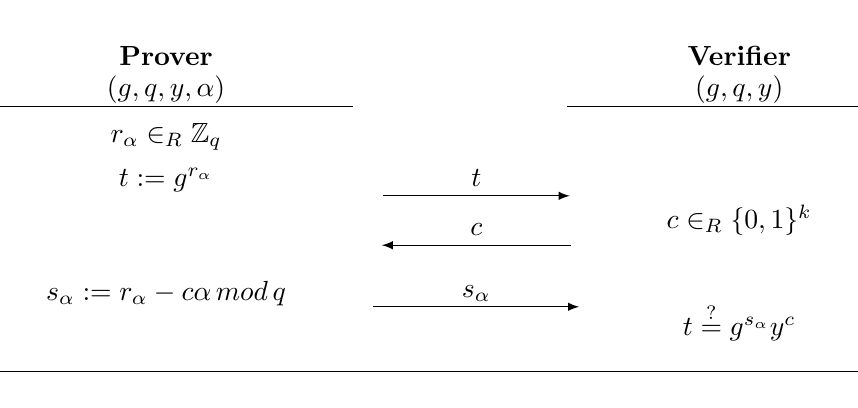
\begin{tikzpicture}
	\matrix (m)[matrix of nodes, column  sep=2cm,row  sep=1mm, nodes={draw=none, anchor=center,text depth=0pt} ]{
		\textbf{Prover} & & \textbf{Verifier}\\[-2mm]
		$(g,q,y,\alpha)$ & & $(g,q,y)$\\%[-4mm]
		$r_\alpha \in_R \mathbb{Z}_q$ & & \\%[-8mm]
		$ t:=g^{r_\alpha} $ & $t$ & \\[-1mm]
		& & $ c \in_R \{0,1\}^{k} $ \\[-4mm]
		& $c$ & \\[2.5mm]
		$ s_\alpha := r_\alpha - c\alpha \, mod\, q $ & $s_\alpha$ & \\[-3mm]
		& & $ t \overset{?}{=} g^{s_\alpha} y^c $ \\
		\hfil & \hfil & \hfil \\
	};
	
	\draw[shorten <=-1.5cm,shorten >=-1.5cm] (m-2-1.south east)--(m-2-1.south west);
	\draw[shorten <=-1.5cm,shorten >=-1.5cm] (m-2-3.south east)--(m-2-3.south west);
	\draw[shorten <=-1cm,shorten >=-1cm,-latex] (m-4-2.south west)--(m-4-2.south east);
	\draw[shorten <=-1cm,shorten >=-1cm,-latex] (m-6-2.south east)--(m-6-2.south west);
	\draw[shorten <=-1cm,shorten >=-1cm,-latex] (m-7-2.south west)--(m-7-2.south east);
	\draw[shorten <=-2.5cm,shorten >=-2.5cm] (m-9-1.south west)--(m-9-3.south east);
	\end{tikzpicture}
\end{document}